\documentclass[tikz]{standalone}
\usepackage[utf8]{inputenc}
\usetikzlibrary{calc,intersections}

\begin{document}

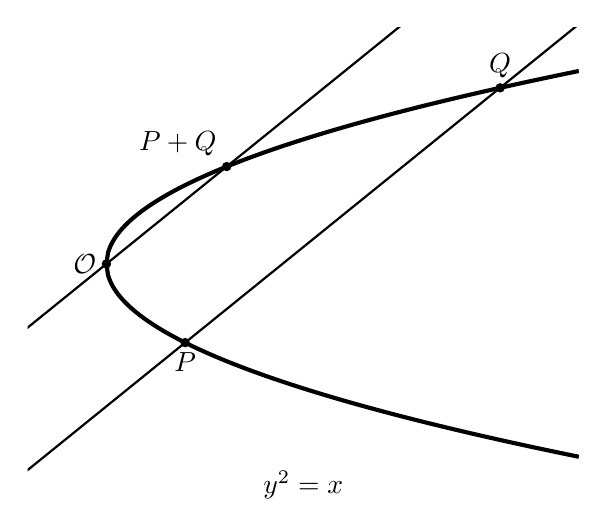
\begin{tikzpicture}[thick,scale=1]
\def\ptsize{.06}
\clip (-1,-3) rectangle (6,3);
\coordinate[label=left:$\mathcal{O}$] (inf) at (0,0);
\path[draw,name path=para1,samples=300,line width=1.5pt,domain=0:6] plot (\x, {sqrt(\x)});
\path[draw,name path=para2,samples=300,line width=1.5pt,domain=0:6] plot (\x, -{sqrt(\x)});
\fill (inf) circle (\ptsize);
\coordinate[label=below:$P$] (P) at (1,-1);
\coordinate[label=above:$Q$] (Q) at (5,{sqrt(5)});
\fill (P) circle (\ptsize);
\fill (Q) circle (\ptsize);
\draw[shorten >=-3cm,shorten <=-3cm] (P) -- (Q);
\path[name path=lineOR,draw,shorten >=-8cm,shorten <=-8cm] (inf) -- +($(P)-(Q)$);

\coordinate[label=above left:$P+Q$] (R) at ({6 - 2*sqrt(5)},{-1 + sqrt(5)});
\fill (R) circle (\ptsize);
\node[below] at (2.5,-2.5) {$y^2 = x$};

\end{tikzpicture}

\end{document}